\documentclass[a4paper, 11pt]{article}

\usepackage{xcolor}
\input{/home/aroquemaurel/cours/includesLaTeX/couleurs.tex}
\usepackage{lmodern}
\usepackage[utf8]{inputenc}
\usepackage[T1]{fontenc}
\usepackage[francais]{babel}
\usepackage[top=1.7cm, bottom=1.7cm, left=2.5cm, right=2.5cm]{geometry}
\usepackage{verbatim}
\usepackage{tikz} %Vectoriel
\usepackage{listings}
\usepackage{fancyhdr}
\usepackage{multido}
\usepackage{amssymb}
\usepackage{multicol}
\usepackage{float}
\usepackage[urlbordercolor={1 1 1}, linkbordercolor={1 1 1}, linkcolor=vert1, urlcolor=bleu, colorlinks=true]{hyperref}

\newcommand{\titre}{Analyse de couverture de coe}
\newcommand{\numero}{2 \& 3}
\newcommand{\typeDoc}{TP}
\newcommand{\module}{Tests et maintenance logiciel}
\newcommand{\sigle}{TML}
\newcommand{\semestre}{6}


\usepackage{ifthen}
\date{\today}

\chead{Antoine de \bsc{Roquemaurel}}
\rhead{TP\no\typeDoc}
\lhead{\titre}
%\makeindex

\lfoot{Université Toulouse III -- Paul Sabatier}
\rfoot{\sigle\semestre}
%\rfoot{}
\cfoot{--~~\thepage~~--}

\makeglossary
\makeatletter
\def\clap#1{\hbox to 0pt{\hss #1\hss}}%

\def\haut#1#2#3{%
	\hbox to \hsize{%
		\rlap{\vtop{\raggedright #1}
	}%
	\hss
	\clap{\vtop{\centering #2}
}%
\hss
\llap{\vtop{\raggedleft #3}}}}%
\def\bas#1#2#3{%
	\hbox to \hsize{%
		\rlap{\vbox{
			\raggedright #1
		}
	}%
	\hss \clap{\vbox{\centering #2}}%
	\hss
	\llap{\vbox{\raggedleft #3}}}
}%
\def\maketitle{%
	\thispagestyle{empty}{%
		\haut{}{\@blurb}{}
		%	
		%\vfill

		\begin{center}
			\vspace{-2.0cm}
			\usefont{OT1}{ptm}{m}{n}
			\huge \@type \@title
		\end{center}
		\par
		\hrule height 1pt
		\par
		\vspace{1cm}
		\bas{}{}{}
}%
}
\def\date#1{\def\@date{#1}}
\def\author#1{\def\@author{#1}}
\def\type#1{\def\@type{#1}}
\def\title#1{\def\@title{#1}}
\def\location#1{\def\@location{#1}}
\def\blurb#1{\def\@blurb{#1}}
\date{\today}
\newboolean{monBool}
\setboolean{monBool}{true}
\author{}
\title{}
\ifthenelse{\equal{\typeDoc}{}}{
\numeroTD{}
}
{
	\type{\typeDoc~--- }
}
\location{Amiens}\blurb{}
%\makeatother
\title{\titre}
\author{%Semestre \semestre
}

\location{Toulouse}
\blurb{%
\vspace{-35px}
\begin{flushleft}
	Université Toulouse III -- Paul Sabatier\\
	L2 Informatique\\
\end{flushleft}
\begin{flushright}
	\vspace{-45px}
	\Large \textbf \module \\
	\normalsize \textit \today\\
	Semestre \semestre
	\vspace{30px}
\end{flushright}
Antoine de \bsc{Roquemaurel}
}%



%\title{Cours \\ \titre}
%\date{\today\\ Semestre \semestre}

%\lhead{Cours: \titre}
%\chead{}
%\rhead{\thepage}

%\lfoot{Université Paul Sabatier Toulouse III}
%\cfoot{\thepage}
%\rfoot{\sigle\semestre}

\pagestyle{fancy}

\input{/home/aroquemaurel/cours/includesLaTeX/listings.tex} %prise en charge du langage C 




%----------------------------------------------------------------------------------------
%	DEFINITION OF COLORED BOXES
%----------------------------------------------------------------------------------------

\RequirePackage[framemethod=default]{mdframed} % Required for creating the theorem, definition, exercise and corollary boxes

% Theorem box
\newmdenv[skipabove=7pt,
skipbelow=7pt,
backgroundcolor=black!5,
linecolor=ocre,
innerleftmargin=5pt,
innerrightmargin=5pt,
innertopmargin=5pt,
leftmargin=0cm,
rightmargin=0cm,
innerbottommargin=5pt]{tBox}

% Exercise box	  
\newmdenv[skipabove=7pt,
skipbelow=7pt,
rightline=false,
leftline=true,
topline=false,
bottomline=false,
backgroundcolor=ocre!10,
linecolor=ocre,
innerleftmargin=5pt,
innerrightmargin=5pt,
innertopmargin=5pt,
innerbottommargin=5pt,
leftmargin=0cm,
rightmargin=0cm,
linewidth=4pt]{eBox}	

% Definition box
\newmdenv[skipabove=10pt,
skipbelow=10pt,
rightline=false,
leftline=true,
topline=false,
bottomline=false,
linecolor=ocre,
innerleftmargin=5pt,
innerrightmargin=5pt,
innertopmargin=0pt,
leftmargin=0cm,
rightmargin=0cm,
linewidth=4pt,
innerbottommargin=0pt]{dBox}	

% Corollary box
\newmdenv[skipabove=7pt,
skipbelow=7pt,
rightline=false,
leftline=true,
topline=false,
bottomline=false,
linecolor=gray,
backgroundcolor=black!5,
innerleftmargin=5pt,
innerrightmargin=5pt,
innertopmargin=5pt,
leftmargin=0cm,
rightmargin=0cm,
linewidth=4pt,
innerbottommargin=5pt]{cBox}		

% Corollary box
\newmdenv[skipabove=7pt,
skipbelow=7pt,
rightline=true,
leftline=false,
topline=false,
bottomline=true,
linecolor=gray,
backgroundcolor=black!5,
innerleftmargin=5pt,
innerrightmargin=5pt,
innertopmargin=5pt,
leftmargin=0cm,
rightmargin=0cm,
linewidth=1pt,
innerbottommargin=5pt]{rBox}				  
		  

% Creates an environment for each type of theorem and assigns it a theorem text style from the "Theorem Styles" section above and a colored box from above
\newenvironment{theorem}{\begin{tBox}\begin{theoremeT}}{\end{theoremeT}\end{tBox}}
\newenvironment{example}{\begin{exampleT}}{\hfill{\tiny\ensuremath{\blacksquare}}\end{exampleT}}
\newenvironment{definition}{\begin{dBox}\begin{definitionT}}{\end{definitionT}\end{dBox}}
\newenvironment{attention}{\begin{eBox}\small}{\end{eBox}}				  	
\newenvironment{exemple}{\begin{cBox}\small}{\end{cBox}}	

%----------------------------------------------------------------------------------------
%	REMARK ENVIRONMENT
%----------------------------------------------------------------------------------------

\newenvironment{remarque}{\par\vskip10pt\small
\begin{rBox}
\begin{list}{}{
\leftmargin=35pt % Indentation on the left
\rightmargin=25pt}\item\ignorespaces % Indentation on the right
\makebox[-2.5pt]{\begin{tikzpicture}[overlay]
\node[draw=ocre!60,line width=1pt,circle,fill=ocre!25,font=\sffamily\bfseries,inner sep=2pt,outer sep=0pt] at (-15pt,0pt){\textcolor{ocre}{R}};\end{tikzpicture}} % Orange R in a circle
\advance\baselineskip -1pt}
{\end{list}\vskip1mm\end{rBox}\vskip5pt} % Tighter line spacing and white space after remark



\input{/home/aroquemaurel/cours/includesLaTeX/polices.tex}
\input{/home/aroquemaurel/cours/includesLaTeX/affichageChapitre.tex}
\makeatother
\begin{document}
	\maketitle

	\section{Algorithme}
	L'algorithme à été développé en java. Afin de créer la liste, deux classes ont été créés : \texttt{List} et \texttt{Cell}. 

	\subsection{\texttt{Cell}}
	\texttt{Cell} est une cellule de la liste, elle contient donc la cellule précédente, la suivante et la valeur concernée\footnote{La valeur est de
	type \texttt{int}}. 

	Cette classe possède la visibilité package afin que celle si ne soit pas utilisée à mauvais escient.

	\lstinputlisting[language=Java, caption=Classe \texttt{Cell}]{src/list/Cell.java}

	\subsection{\texttt{List}}
	La classe \texttt{List} qui est publique, permet à l'utilisateur de créer une liste triée et d'y ajouter des éléments\footnote{Possibilité d'ajouter
	un élément depuis la méthode \texttt{add} ou depuis le constructeur}.

	L'algorithme proposé à donc été implémenté dans la méthode \texttt{add}.
	\lstinputlisting[language=Java, caption=Classe \texttt{List}]{src/list/List.java}

	\section{Instructions couvrant une insertion en position intermédiaire}
	\subsection{Ajout des deux premiers entiers}
	Figure \ref{fig:1erEntiers} est disponible la couverture pour l'insertion des deux premiers entiers, avant l'insertion de l'entier qui nous
	intéresse.

	\begin{figure}[H]
		\centering
		\includegraphics[width=7.5cm]{screens/ajout1-5.png}
		\label{fig:1erEntiers}
		\caption{Ajout des entiers 1 et 5 dans une liste vide}
	\end{figure}

	\subsection{Ajout de l'entier 4}
	Afin d'insérer l'entier 4, les entiers 1 et 5 devaient être déjà présents dans la liste, afin
	d'éviter que le rapport d'emma soit faussé par ces deux insertions, une nouvelle méthode à été créé insérant ces deux entiers.

	\begin{figure}[H]
		\centering
		\includegraphics[width=7.5cm]{screens/ajout4.png}
		\label{fig:entier4}
		\caption{Ajout de l'entier 4 dans une liste possédant 1 et 5}
	\end{figure}
	
	Comme le montre la figure \ref{fig:entier4}, l'insertion du 4 ne passe que par une portion du code, en effet, les instructions d'insertion en tête
	ou en queue ne sont pas nécessaire ici, c'est ainsi que la condition \texttt{current != null} du while et le test \texttt{previous == null} ne sont
	pas nécessaire pour l'insertion intermédiaire. Nous pouvons observer avec la figure \ref{fig:1erEntiers} que l'insertion en tête ou en queue à
	l'inverse passe dans ces deux instructions mais n'a pas besoin du test vérifiant si \texttt{current.getData() > data}.

	On peut donc en déduire que c'est ce test qui permet à l'insertion intermédiaire de fonctionner : ça permet d'insérer notre élément à une place
	correct dans la liste triée.
	\section{Jeu de test minimal}
	Afin de pouvoir tester toutes les instructions du
	programme, il faut utiliser un jeu de test gérant tous
	les cas possibles. 

	Pour l'insertion dans une liste, 3 cas ressortent et sont
	donc représentés dans le code : insertion en début de
	liste, insertion en fin de liste, insertion en position
	intermédiaire. Ainsi, notre jeu de test devra comporter 3
	entiers afin de tester ces trois cas.

	\begin{description}
		\item[Insertion en début] 1
		\item[Insertion en queue] 20
		\item[Insertion en position intermédiaire] 4
	\end{description}

	L'insertion consécutive de ces 3 entiers ci-dessous
	couvriront l'intégralité du code comme le montre la
	figure \ref{fig:couvmin1}

	\begin{figure}[H]
		\centering
		\includegraphics[width=13cm]{screens/testMin1.png}\\
		\includegraphics[width=6cm]{screens/testMin2.png}
		\includegraphics[width=6cm]{screens/testMin3.png}
		\label{fig:couvmin1}
		\caption{Tests de couverture avec un jeu de test minimal}
	\end{figure}
	\newpage
	\begin{remarque}
		Le fichier de Test ne possède pas 100\% de couverture
		car nous n'utilisons que le \texttt{main} et pas la
		classe qui le contient.

		Cependant, cela n'est pas important car nous testons
		le package \texttt{list}, celui-ci possède bien
		100\%.
	\end{remarque}

	\section{Cas d'insertion et instructions}
	Oui, la couverture de toutes les instructions permettent ici de tester les cas possible.

	En effet, notre fonction d'insertion possède différentes conditions en fonction du placement du chiffre :

	\begin{description}
		\item[Insertion en début] Nous ne rentrons pas dans la boucle, et passons dans le cas \texttt{previous == null} afin d'affecter la tête
			à courant.
		\item[Insertion en position intermédiaire] C'est le seul cas permettant de vérifier que nous sortons bien de la boucle avant la fin : 
			ce qui nous permet d'insérer ensuite notre entier au milieu de la liste. Ceci est fait grâce à la condition \texttt{current.getData() > data}.
		\item[Insertion en queue] C'est le cas ou l'intégralité de la boucle est parcourue, afin de vérifier que nous sortons bien de la boucle une
			fois la fin de liste atteint. C'est l'instruction \texttt{current != null} qui est dans le test de la boucle.
	\end{description}

	Nous testons tous les cas possibles, cependant nos tests ne permettent pas de dire si la liste en sortis est bien triée, en effet, rien ne nous
	permet de dire si les entiers sont insérés au bon endroit.

	\section{Graphe de contrôle et PLCS}
	\subsection{Graphe de contrôle}
	Figure \ref{fig:graphe} est disponible le graphe de contrôle du programme, en utilisant le constructeur permettant une insertion multiple.

	\begin{figure}[H]
		\centering
		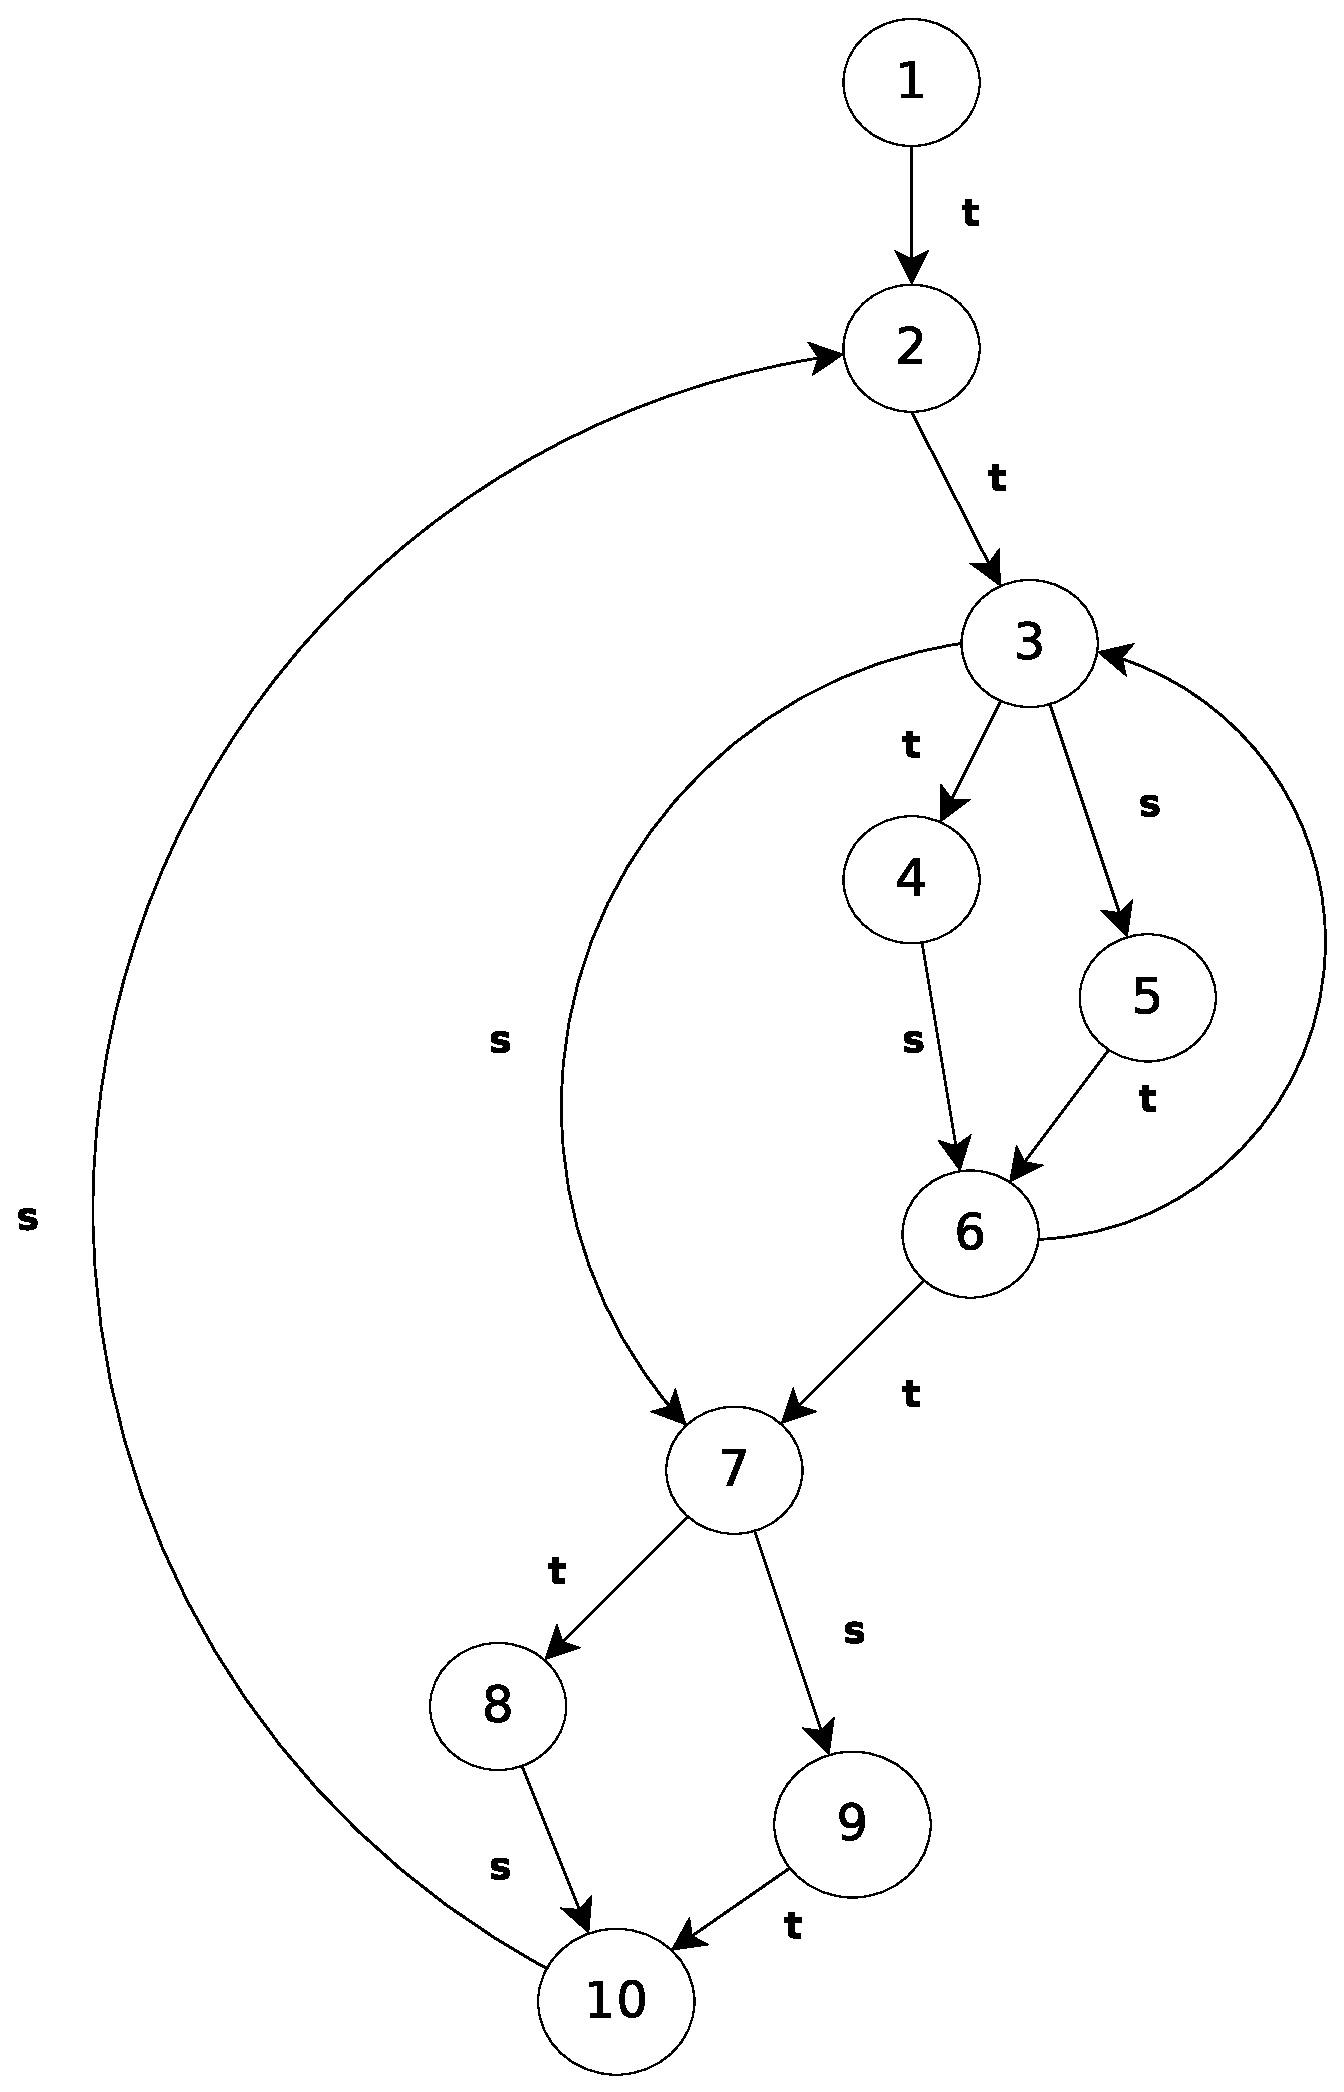
\includegraphics[width=7cm]{Diagramme.eps}
		\caption{Graphe de contrôle}
		\label{fig:graphe}
	\end{figure}
	\subsection{PLCS}
	\begin{itemize}
		\item 1\&2\&3\&4,6
		\item 1\&2\&3, 5
		\item 1\&2\&3,7
		\item 2\&3, 5
		\item 2\&3,7
		\item 2\&3\&4,6	
		\item 3,7
		\item 3\&4,7
		\item 3,5
		\item 5\&6\&7,9
		\item 5\&6,3
		\item 5\&6\&7\&8,10
		\item 6\&7\&8,10
		\item 6\&7,9
		\item 6,3
		\item 7,9
		\item 7\&8,10
		\item 9\&10,2
		\item 9\&10,-1
		\item 10, -1
	\end{itemize}
	
\end{document}
